\documentclass{article}
\date{}
\usepackage[margin=1in]{geometry}
\usepackage{amsmath,amssymb}
\usepackage{verbatim}
\usepackage{pdflscape}
\usepackage{graphicx, subfigure}
\usepackage{adjustbox}

\providecommand{\keywords}[1]{\textbf{\textit{Keywords ---}} #1}

\begin{document}
\title{Wisdom of the Crowds: Survey Results}
\maketitle




\section*{Overview of Experiment}

Five questions were asked during the introduction to the wisdom of the crowd experiment. They were as follows: 
\begin{itemize}
\item What is the total area of India in km$^{2}$?
\item In what year was the painting made? 
\item How many dots are in the figure?
\item How many runs will India score in the upcoming cricket match?
\item How many runs will Pakistan score in the upcoming cricket match?
\end{itemize}

The painting question was a multiple choice question where participants were asked to choose between four possible years. All others were open-ended where participants were asked to enter text. \\


\section*{Data Preprocessing and Outlier Detection}

Visual inspection of the data exhibited obviously erroneous data points for two of the tasks which had to be removed prior to proceeding with the data analysis. These were mostly due to incorrect units used (eg. Lakhs instead of Km), or participants submitting answers before the images were shown and explained (eg. answers of 0 dots). For the number of dots question, observations less than 10 were removed (4 observations). For the landmass of India question, observations less than 100 were removed (1 observation).\\

After discarding these values, we use the standard interquartile range method to identify outliers. The interquartile range (IQR) is given by the difference between the third and first quantiles, Q$_{3}$ - Q$_{1}$. Any value that falls outside the range $\left\{ Q_{1} - 1.5*\text{IQR}, Q_{3}+1.5*\text{IQR} \right\}$ is a suspected outlier. 


\section*{Summary Statistics}

The summary table below represent survey results after the removal of outliers. For the mean, truncated mean and geometric mean, the percent of responses that are worse than the crowd estimate is included in parenthesis. \\

The histograms in Figures 1-4 show the distribution of the responses. The red line indicates the correct answer and the dotted blue line indicates the average guess of participants.


\begin{table}[h]
\begin{adjustbox}{max width=\textwidth}
\begin{tabular}{|l||r|r|r|r|r||r|r|r|r|r|}
\hline
Task & Correct value & Median & Mean & 25\% Trunc mean & Geometric mean & Nr of responses	& Min & Max & 	St.Dev & Skewness \\
\hline
Nr Dots & $1,149$ & $587.5$ & $812.2$ & $ 635.7 $ & $422.5$ & 76 & 10 & $3,000$ & $769.6$ & $1.2$ \\
& & & (80\%) & (68\%) & (57\%) & & & & &  \\
Yr Painting & $1890$ & 1820 & $1847.8$ & $1848.5$ & $1847.8$ & 83 & 1750 & 1960 & $63.7$ & $0.2$ \\
& & & (71\%) & (71\%) & (71\%) & & & & &  \\        
Runs India & $300$ & $280$ & $282.8$ & $ 283.6$ & $281.9$ & 78 & $200$ &	$368$	& $32.7$ & $0.1$ \\
& & & (71\%) & (71\%) & (71\%) & & & & &  \\   
Runs Pakistan & 224	& 256 & $253.2$ & $253.8$ & $251.9$ & $77$ & $175$ & $340$ & $33.9$ & $-0.1$ \\
& & & (55\%) & (55\%) & (55\%) & & & & &  \\   
Landmass India & $3,287,590$ & $1,000,000$ & $2,077,340$ &	 $1,355,714.2$ & $475,902$	& $71$ & $100$ &	 $10,000,000$ & $2,472,027$ & $1.6$ \\
& & & (77\%) & (63\%) & (41\%) & & & & &  \\
\hline
\end{tabular}
\end{adjustbox}
\caption{Summary Statistics}
\label{stats}
\end{table} 


				
\newpage

\begin{figure}
\begin{center}
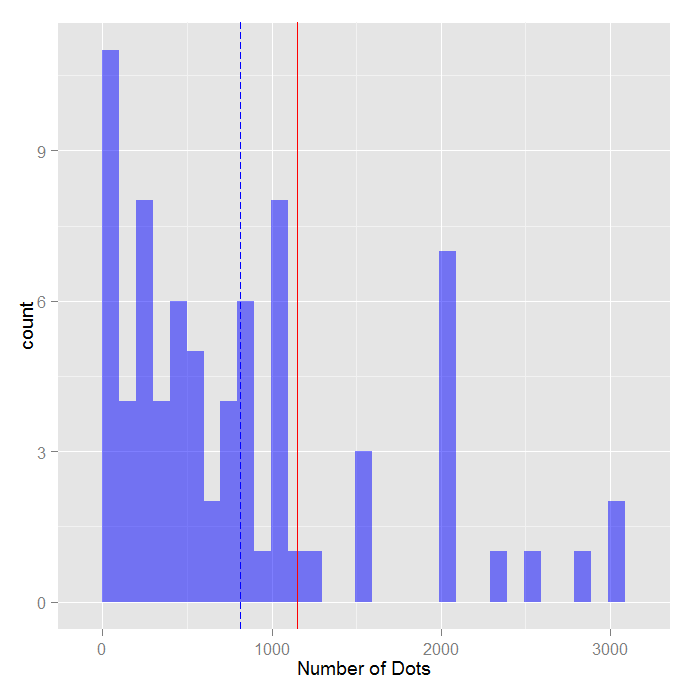
\includegraphics[width=0.65\textwidth]{nrDots.png}
\caption{Distribution of guesses for the number of dots}
\label{nrDots}
\end{center}	
\end{figure}




\begin{figure}
\begin{center}
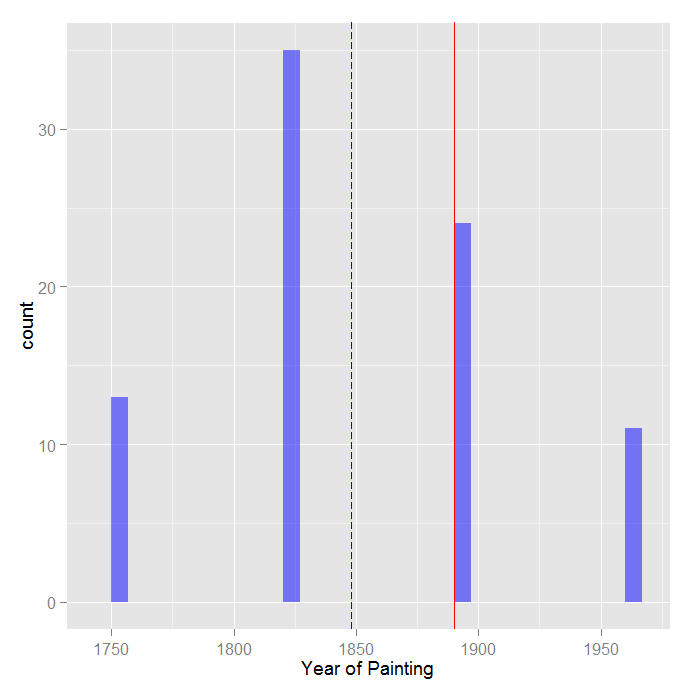
\includegraphics[width=0.65\textwidth]{year.png}
\caption{Distribution of guesses for the year of painting}
\label{painting}
\end{center}	
\end{figure}





\begin{figure}[ht!]
     \begin{center}
        \subfigure[]{
            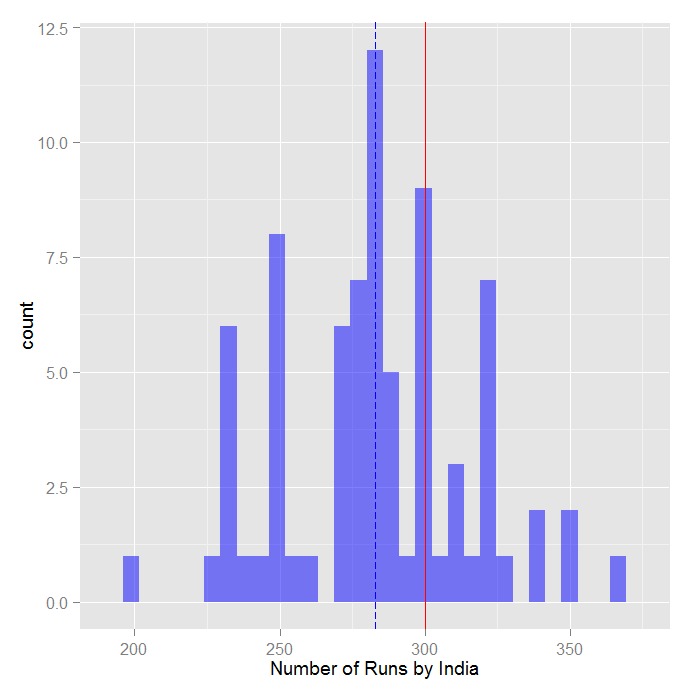
\includegraphics[width=0.45\textwidth]{runsIndia.png}
            \label{India}
        }
        \subfigure[]{
           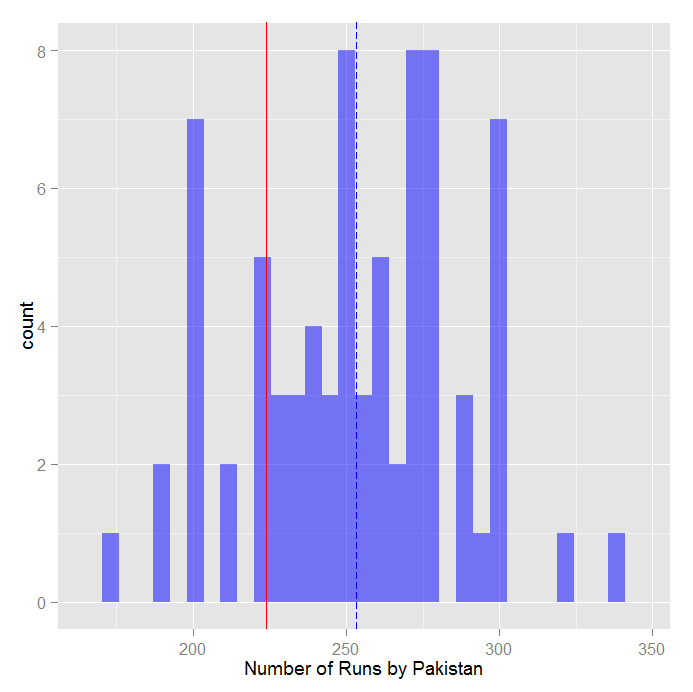
\includegraphics[width=0.45\textwidth]{runsPakistan.png}
           \label{Pakistan}
		}
    \end{center}
    \caption{Distribution of guesses for the number of runs for India \ref{India} and Pakistan \ref{Pakistan}.}
\end{figure}


\begin{figure}
\begin{center}
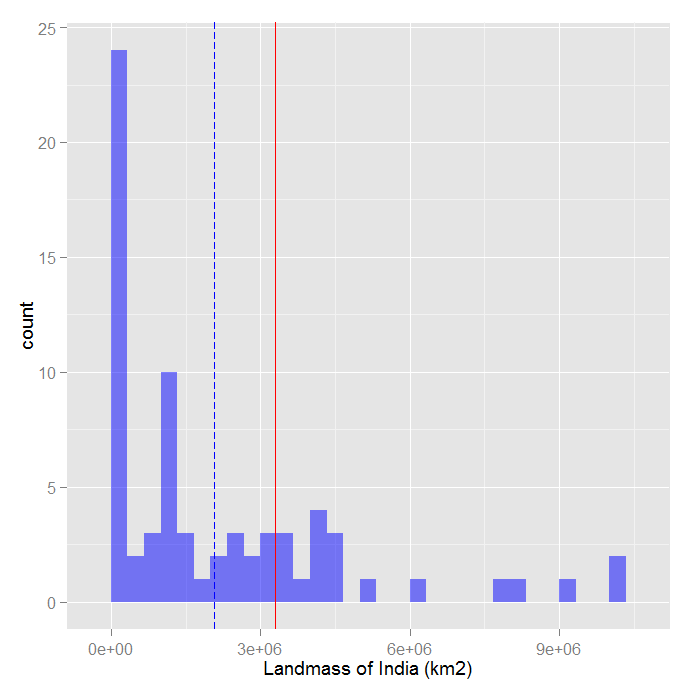
\includegraphics[width=0.65\textwidth]{indiaTerritory.png}
\caption{Distribution of guesses for the landmass of India}
\label{pareto}
\end{center}	
\end{figure}



\end{document}
